\subsection{Embedded Multicore Building Blocks}
\begin{frame}
	\frametitle{\secname}
	\framesubtitle{\subsecname}
	
	\begin{itemize}
		\item von Siemens entwickelt
			\note[item]{ab 1.10.2014 Open Source, aktuell 0.3.0 vom 27. Mai}
		\item vor allem für Embedded Systeme
			\note[item]{aber auch für normale Software geeignet}
		\item C/C++
			\note[item]{}
		\item Ziel: Abstraktion von (low-Level) Thread-Management
			\note[item]{man muss sich nicht mehr selber drum kümmern}
		\item Unterstützt Task Prioritäten
			\note[item]{hat geheißen, das machen nicht viele}
		\item Aufgebaut auf MTAPI
		\begin{itemize}
			\item standardisiertes Programminterface
				\note[item]{um Parallelisierung auf Embedded Systeme zu bringen}
			\item Unterstützt symmetrische und asymmetrische Prozessoren
				\note[item]{asymmetrische: nicht alle haben gleiche Priorität/Aufgabenverteilung, z.B. nur einer kann Betriebssystem-Code ausführen}
		\end{itemize}
	\end{itemize}
\end{frame}

\subsection{Struktur}
\begin{frame}
	\frametitle{\secname}
	\framesubtitle{\subsecname}
	
	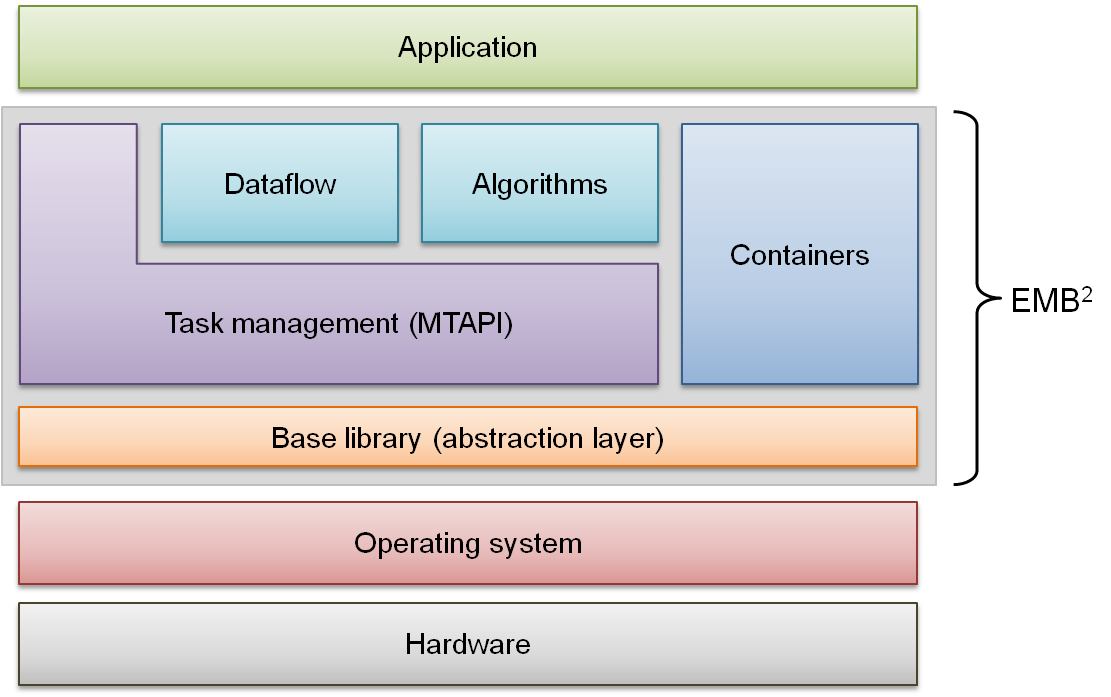
\includegraphics[width=\textwidth]{embb.png}
		\note[item]{oben Applikation, die die Bibliothek benutzt}
		\note[item]{eigentliche Bib, setzt auf MTAPI für die Taskverwaltung auf}
		\note[item]{bietet zusätzliche Klassen und Funktionen, für viel genutzte Algorithmen}
		\note[item]{bietet auch eigene Containerklassen, deren Funktionen parallel bearbeitet werden}
		\note[item]{läuft auf den verschiedensten Prozessorarchitekturen (x86, ARM)}
\end{frame}

\subsection{Beispiel}
\begin{frame}
	\frametitle{\secname}
	\framesubtitle{\subsecname}
	
	Code
		\note{zu lang $\to$ Codeblocks}
\end{frame}